\section{Introduction et motivation}

\begin{frame}
\frametitle{Introduction}
\framesubtitle{Les ondes spirales cardiaques}
%\begin{columns}
%\column{0.55\textwidth}
%\begin{small}
%\begin{itemize}
%  \item Les arythmies cardiaques, comme la tachycardie ventriculaire et la fibrillation, sont des troubles du rythme qui peuvent entraîner une mort subite en quelques minutes.
%  \item Dans de nombreux cas, ces arythmies sont entretenues par une onde électrique auto‑entretenue qui tourne dans le muscle cardiaque : une onde spirale.
%  \item Modéliser ce phénomène permet d’en comprendre les mécanismes profonds et d’envisager des stratégies thérapeutiques pour interrompre ces ondes, par exemple par défibrillation électrique.
%\end{itemize}
%\end{small}

%\column{0.45\textwidth}
\centering
\begin{figure}
\caption{Onde spirale simulée dans un tissu cardiaque virtuel}
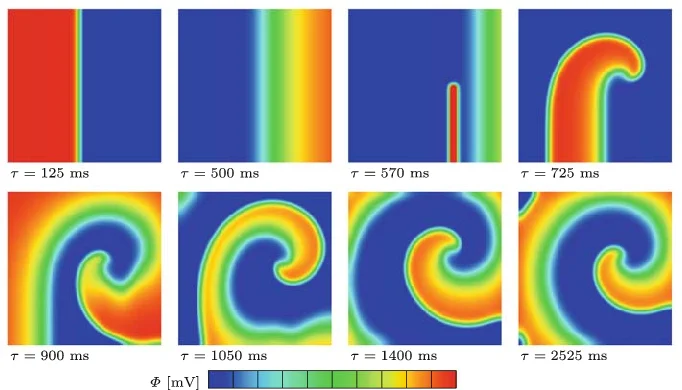
\includegraphics[scale = 0.32]{Figures/onde_spirale_intro.png}
\source{Atrial and ventricular fibrillation: Computational simulation of spiral waves in cardiac tissue}
\end{figure}
%\end{columns}
\end{frame}